\begin{figure}[H]
    \captionsetup[subfigure]{labelformat=empty}
    \begin{subfigure}[t]{0.47\textwidth}
        \begin{subfigure}[t]{0.49\textwidth}
            \caption{A}
            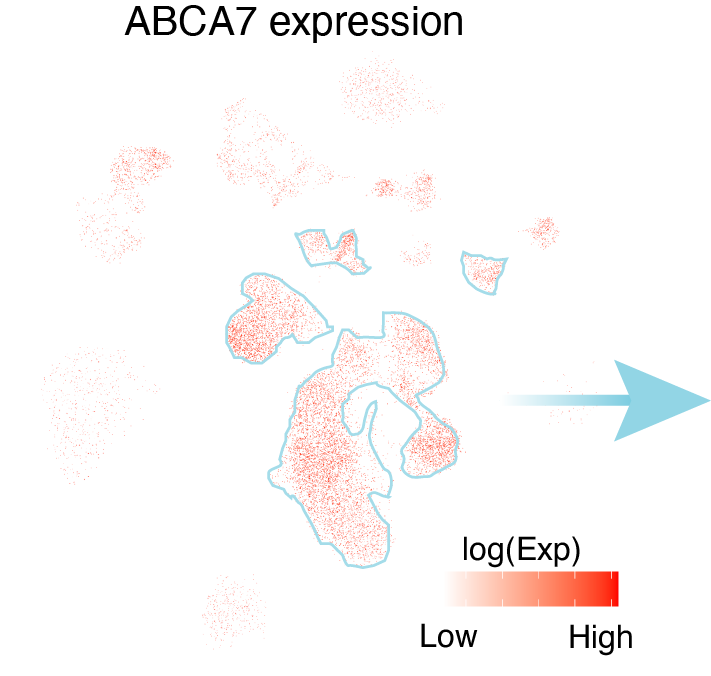
\includegraphics[width=\textwidth]{./main_plots/cell_projection_abca7_expression.png}        
        \end{subfigure}
        \begin{subfigure}[t]{0.49\textwidth}
            %\caption{}
            \vspace{1cm}
            \includegraphics[width=\textwidth]{./main_plots/pm_kl_network_network.pdf}        
        \end{subfigure}
        \begin{subfigure}[t]{\textwidth}
            \caption{C}
            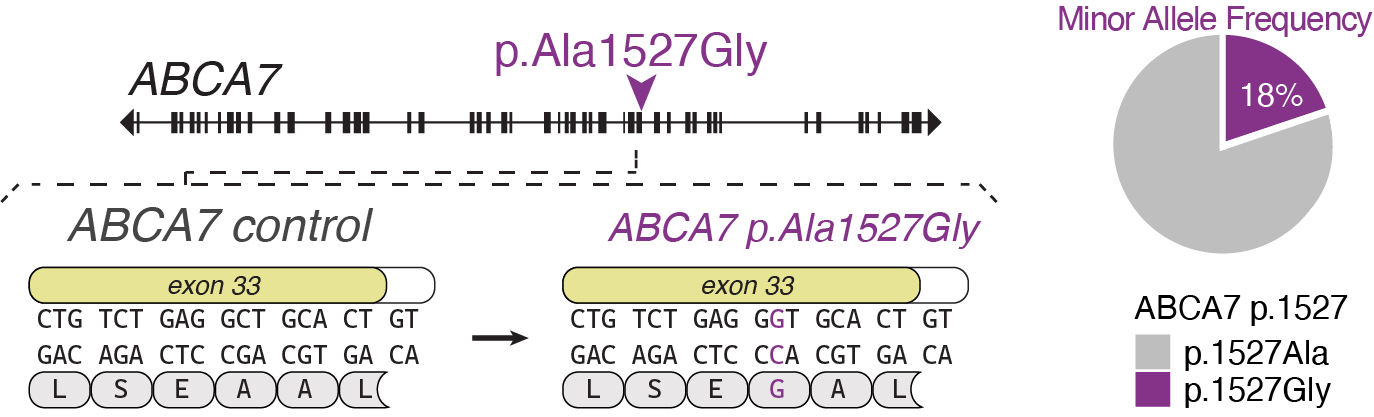
\includegraphics[width=\textwidth]{./main_plots/common_variant_cartoon.png}        
        \end{subfigure}
    \end{subfigure}
    \begin{subfigure}[t]{0.45\textwidth}
        \caption{B}
        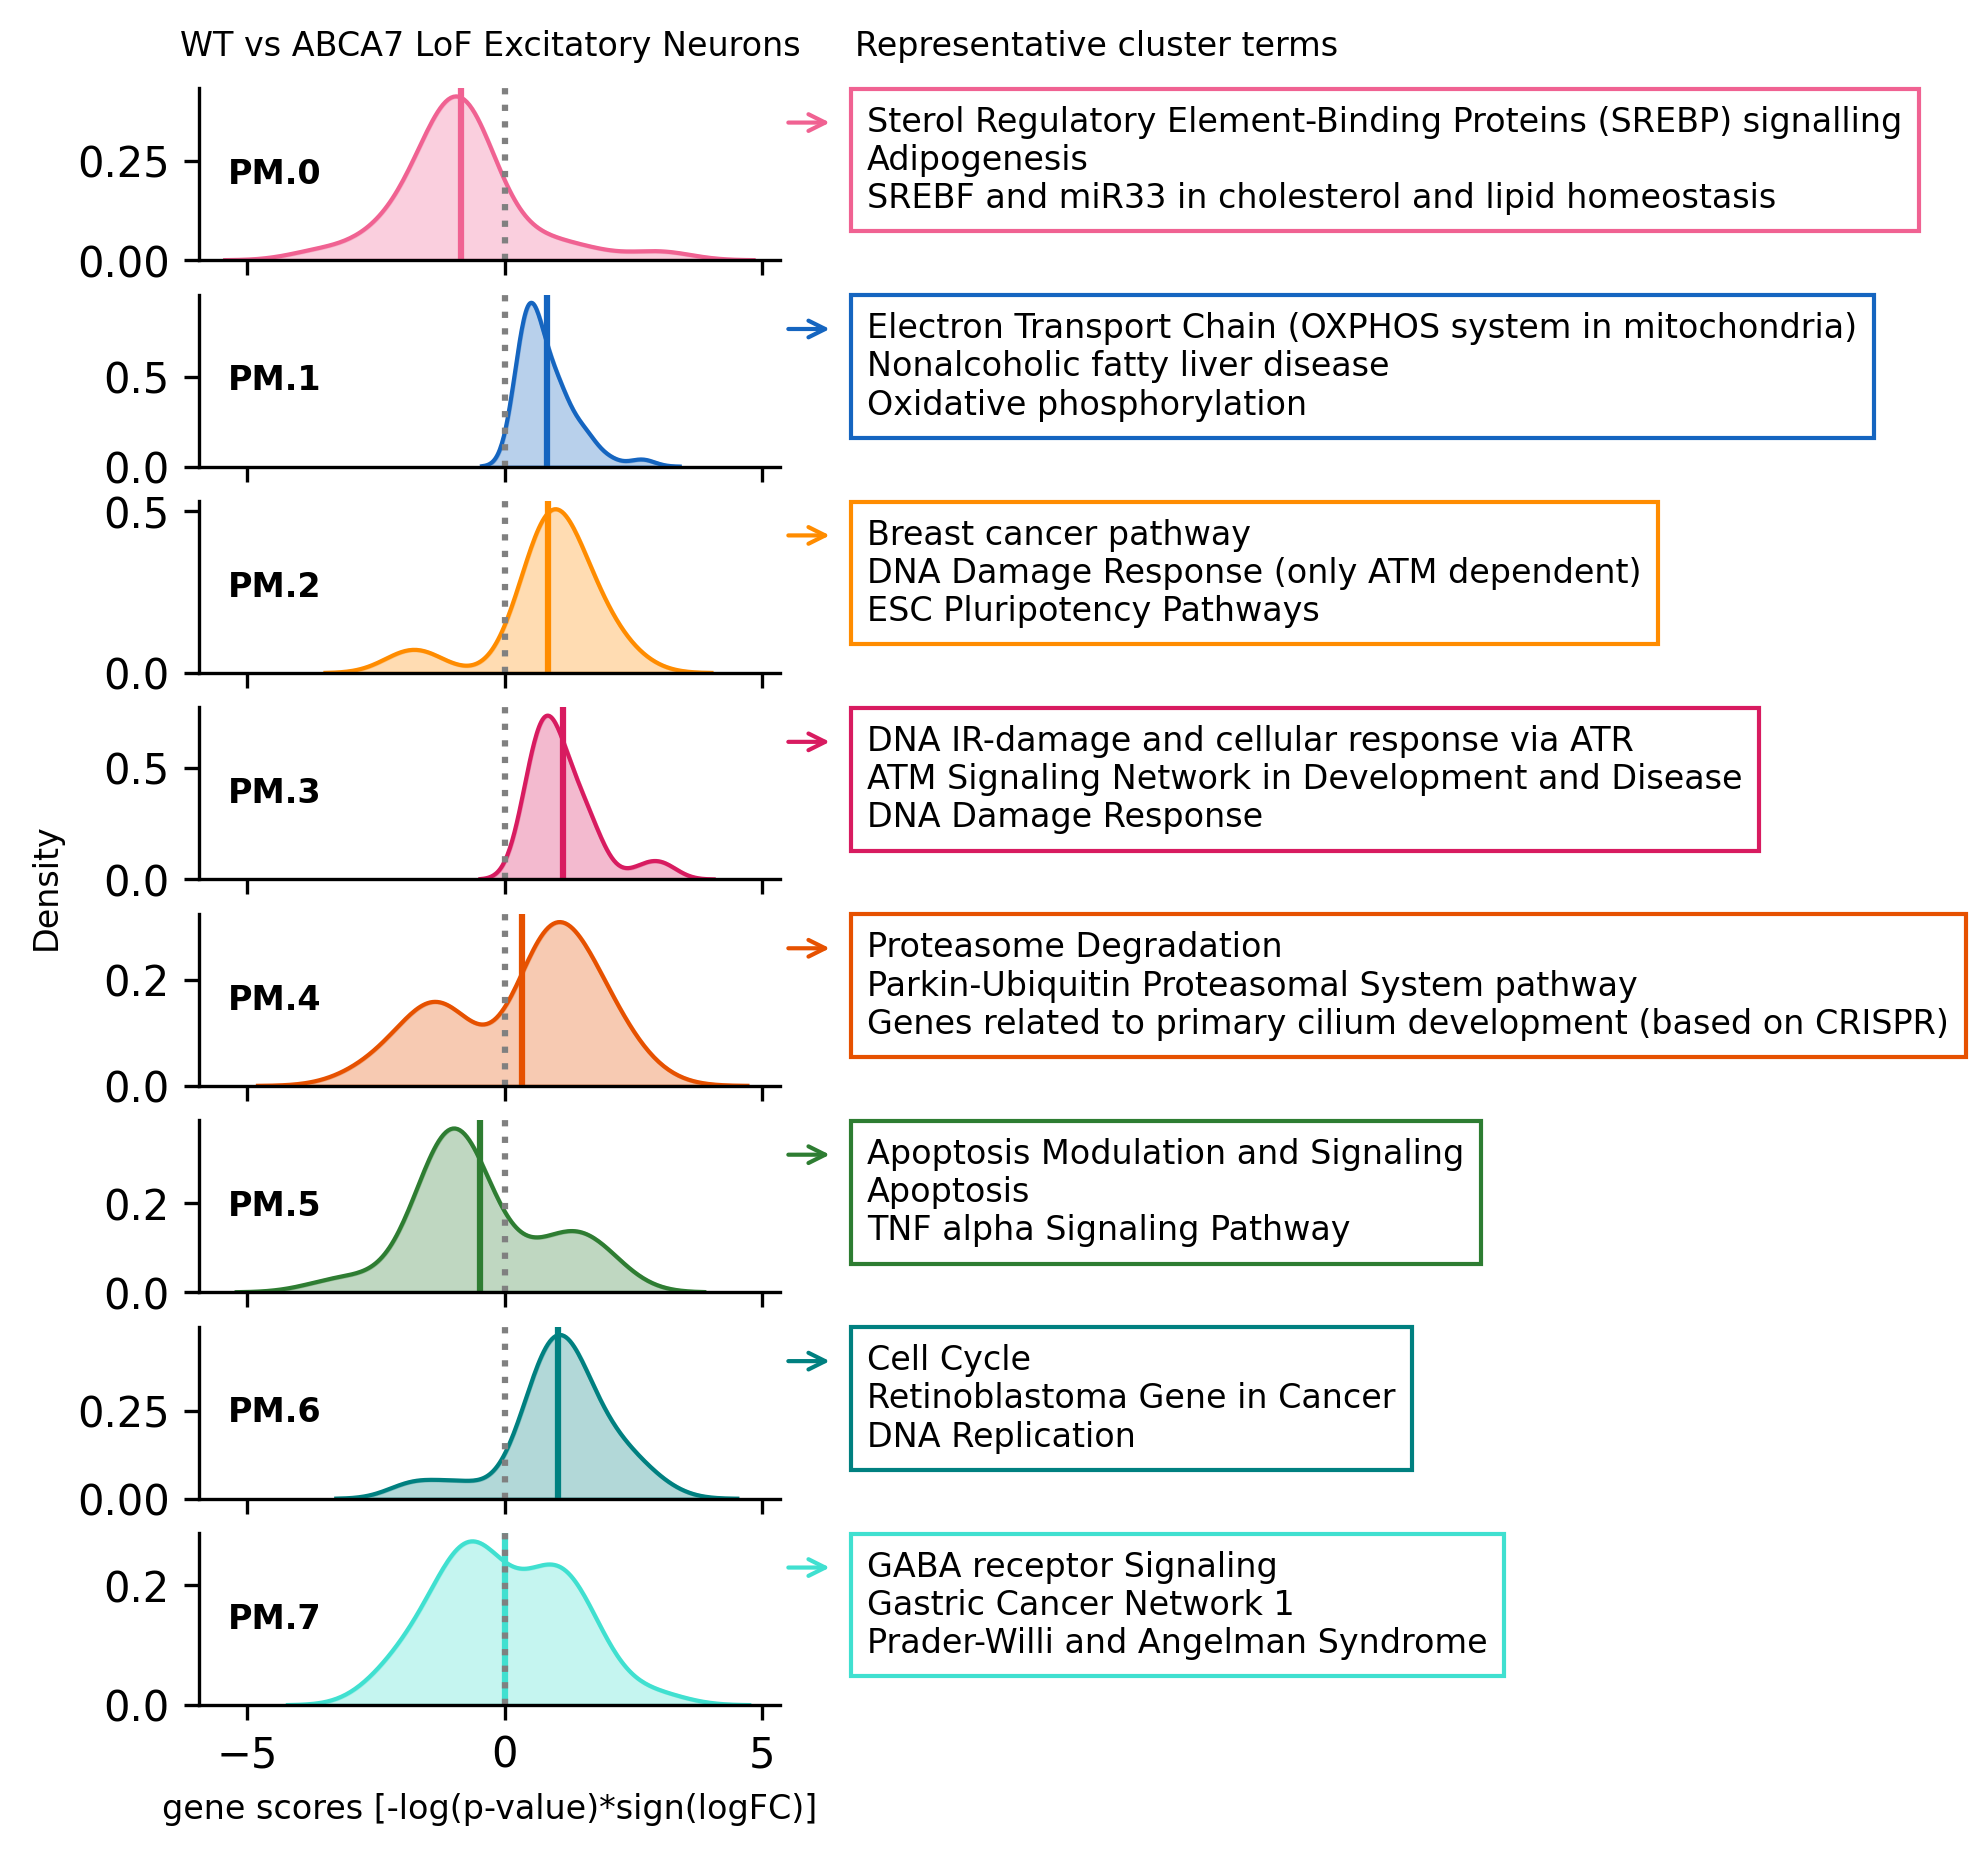
\includegraphics[width=\textwidth]{./main_plots/kl_densities.png}        
    \end{subfigure}
    \begin{subfigure}[t]{0.3\textwidth}
        \caption{D}
        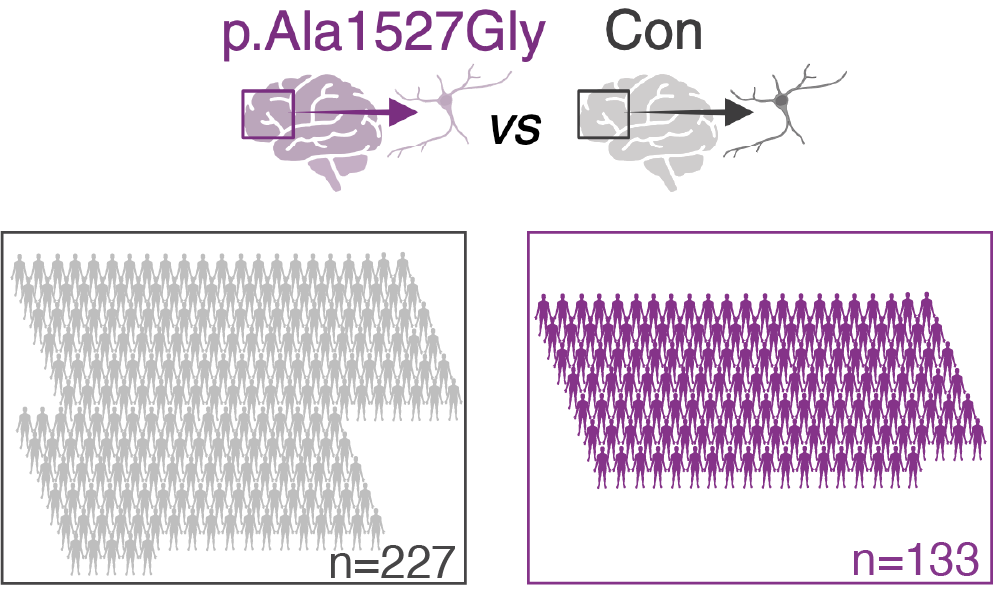
\includegraphics[width=\textwidth]{./main_plots/common_var_cohort_cartoon.png}        
    \end{subfigure}
    \hspace{0.01\textwidth} % Adjust this value as needed
    \begin{subfigure}[t]{0.225\textwidth}
        \caption{E}
        \includegraphics[width=\textwidth]{./main_plots/rs3752246_fgsea_barplot.png}        
    \end{subfigure}
    \begin{subfigure}[t]{0.45\textwidth}
        \caption{F}
        \includegraphics[width=\textwidth]{./main_plots/common_variant_boxplot.png}        
    \end{subfigure}
    \begin{subfigure}[t]{0.3\textwidth}
        \caption{G}
        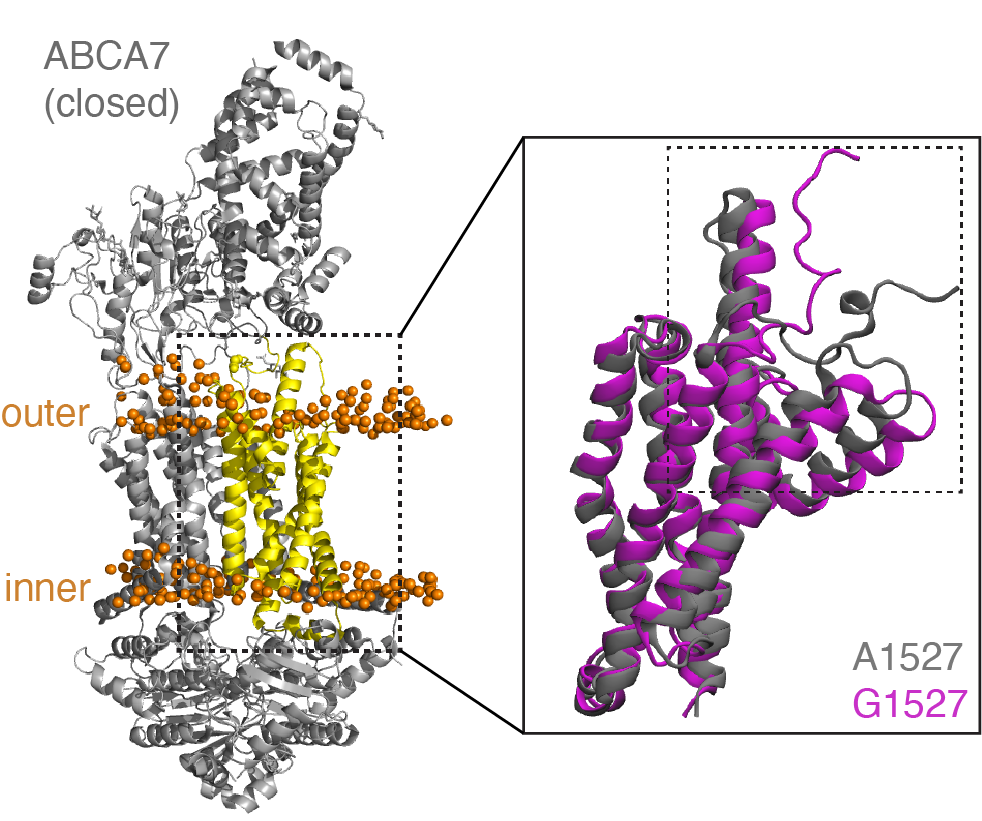
\includegraphics[width=\textwidth]{./main_plots/abca7_structure_with_inset.png}        
    \end{subfigure}
    \begin{subfigure}[t]{0.165\textwidth}
        \caption{H}
        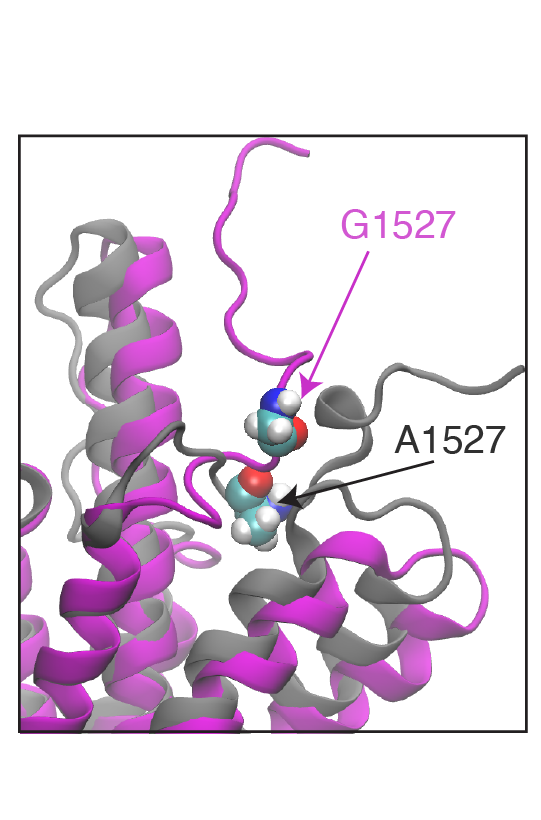
\includegraphics[width=\textwidth]{./main_plots/abca7_inset_only.png}        
    \end{subfigure}
    \hspace{0.01\textwidth} % Adjust this value as needed
    \begin{subfigure}[t]{0.32\textwidth}
        \caption{I}
        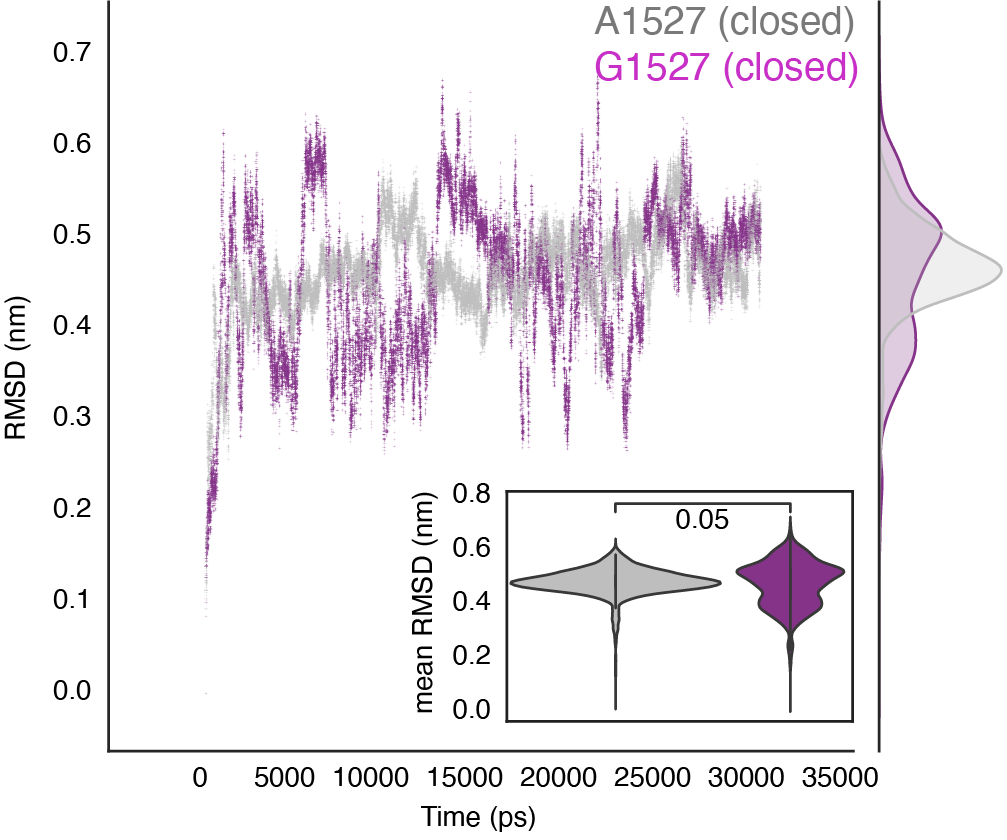
\includegraphics[width=\textwidth]{./main_plots/variant_dynamics.png}        
    \end{subfigure}
    \begin{subfigure}[t]{0.16\textwidth}
        \caption{J}
        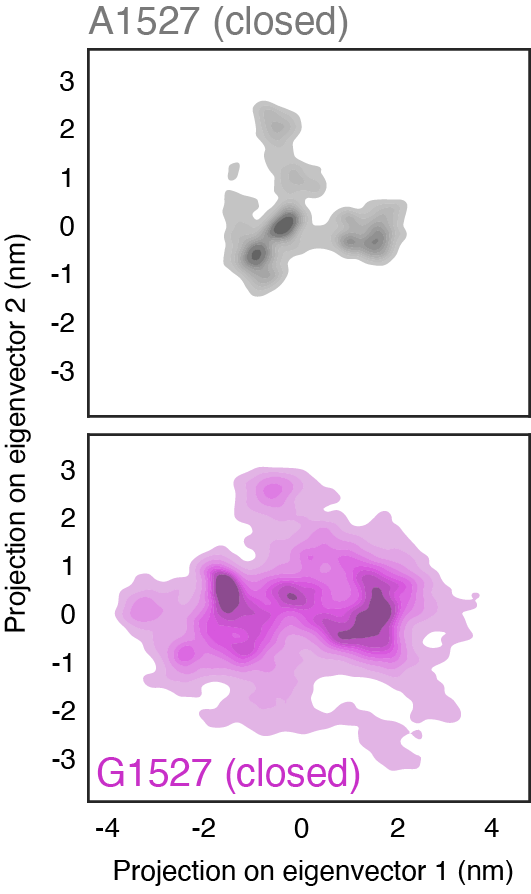
\includegraphics[width=\textwidth]{./main_plots/variant_projection_closed.png}        
    \end{subfigure}
    \caption{
        \textbf{Transcriptional Perturbations in Excitatory Neurons in ABCA7 LoF and ABCA7 p.Ala1527Gly Variant Carriers.}\\
    }
    \label{fig:main_neurons}
\end{figure}
\begin{itemize}
    \item[\textbf{(A)}] (left) 2D UMAP projection colored by log-transformed values of log-normalized ABCA7 expression ($\log(\text{Exp})$). (right) Kernighan-Lin (K/L) clustering of leading-edge genes from significantly perturbed pathways ($p<0.05$) in ABCA7 LoF excitatory neurons. Colors indicate distinct K/L clusters (0–7).
    \item[\textbf{(B)}] Gaussian kernel density plots of gene perturbation scores ($S=-\log_{10}(p)\times\text{sign}(\log_2(\text{FC}))$) per K/L cluster. Positive $S$ indicates upregulation in ABCA7 LoF. Solid lines show distribution means. Representative pathways with highest intra-cluster connectivity annotated per cluster.
    \item[\textbf{(C)}] Schematic of ABCA7 gene highlighting the p.Ala1527Gly codon change (purple arrow). Minor allele frequency (MAF) shown at right.
    \item[\textbf{(D)}] Overview of snRNA-seq cohort comparing ABCA7 p.Ala1527Gly carriers (homozygous/heterozygous) to non-carrier controls (MAF $\approx18\%$).
    \item[\textbf{(E)}] Perturbation (FGSEA scores) of ABCA7 LoF-associated gene clusters from (B) in excitatory neurons from p.Ala1527Gly carriers vs. controls. Top $p$-values ($p<0.1$) indicated. Positive scores represent upregulation in carriers.
    \item[\textbf{(F)}] Distribution of gene perturbation scores ($S$) for each K/L cluster comparing ABCA7 p.Ala1527Gly (no fill) vs. LoF variants (solid fill). Positive $S$ indicates upregulation.
    \item[\textbf{(G)}] Closed-conformation ABCA7 protein structure, highlighting domain (residues 1517–1756, yellow) used for molecular simulations. Lipid bilayer shown in orange. Expanded inset highlights Ala1527 (light grey) and Gly1527 (purple) residues.
    \item[\textbf{(H)}] Expanded inset from (G) with residues of interest indicated.
    \item[\textbf{(I)}] Root mean squared deviations (RMSD) of the closed-conformation ABCA7 domain (G) carrying Ala1527 (light grey) or Gly1527 (purple) during simulation, relative to reference closed conformation. Inset violin plot shows average $C_\alpha$ atom positional fluctuations.
    \item[\textbf{(J)}] Projection of $C_\alpha$ positional fluctuations onto the first two principal components during simulation for Ala1527 (top, light grey) and Gly1527 (bottom, purple).
\end{itemize}